\title{Language Study, Part I} \author{
        Martin Kozeny\\
        CSCI 4501: Programming Language Structure\\
        Spring 2011
        University of New Orleans
}
\date{\today}




\documentclass[5pt]{article}
\usepackage{graphicx}
\usepackage{amssymb}
\usepackage{amsmath}
\usepackage{qtree}
\usepackage{multicol}
%\usepackage{chemarrow}
\usepackage[utf8]{inputenc}
\usepackage{listings}
  \usepackage{courier}
 
 \lstset{
language=C,
basicstyle=\small\sffamily,
numbers=left,
numberstyle=\tiny,
%frame=tb,
columns=fullflexible,
showstringspaces=false
%keywordstyle=[1]\textmd
%tabsize=2, that
}

 \lstloadlanguages{% Check Dokumentation for further languages ...
         %[Visual]Basic
         %Pascal
         C
         %C++
         %XML
         %HTML
         %Lisp
         %Java
 }

\setlength{\hoffset}{-2.3cm} 
\setlength{\voffset}{-3cm}
\setlength{\textheight}{24.0cm} 
\setlength{\textwidth}{16cm}


\begin{document}

\maketitle


\begin{enumerate}
  \item
  \begin{description}
  \item[a]\textbf{Date of first release of the language.}\\
  \\
  According to \cite{krasner:bits_of_history}, Smalltalk-80 system has its roots in the Xerox Palo Alto Research
Center starting more than 10 years ago. Because of publishing book in 1982,
first release of Smalltalk was in 1972 (Smalltalk-72) (page 3). Some others
sources pointed to year 1971.
  \item[b]\textbf{Name of designer or designers.}\\
  \\
  As presented in \cite{wiki:smalltalk}, designers of language are Alan Kay, Dan
  Ingalls, Adele Goldberg, Ted Kaehler, Scott Wallace.
  \item[c]\textbf{Is the actual language version you are using the original
  version? an extension of it? a subset of it? neither an extension nor a subset but a version based on the original language? Explain
your answer.}\\
\\
According to \cite{black:squeak_by_example}, Squeak is a modern,
open source, fully-featured implementation of the Smalltalk programming language and environment so its version based on on the
original language (page ix).
  \item[d]\textbf{If not the original version, state the date of the release of
  the version you are using, as well as the date of the release of the
  translator (compiler, interpreter) you are using to write programs.}\\
  \\
  On \date{October 1 1996}, Dan Ingalls, as he wrote it in
  \cite{ignalls:report}, annouced to the world existence of the new
  implementation of Smalltalk called Squeak. I am using interpreter Squeak 3.9
  released in October 2006 according to \cite{web:squeak}.
  \item[e]\textbf{Do the language have an standard? if so, state release date,
  and state whether the translator you are using implements the standard.}\\
  \\
  According to \cite{web:squeak}, the ANSI Smalltalk standard was approved on
  May 19, 1998. The official name of the document is ANSI INCITS 319-1998 (R2002). The Squeak
  Virtual Machine of Squeak broadly follows the specification of chapter 27 of
  the \cite{goldberg:blue_book}.
  \item[f]\textbf{If the language does not have a standard,}
  \begin{description}
  \item[i]\textbf{list the documents you are using for the release you are
  using.}
  \item[ii]\textbf{how do all the 3 different main language users (language
  designers, language implementors, and programmers) deal with the understanding
  of the language features and their semantics without a standard?}
  \end{description}
  \item[g]\textbf{What programming paradigms does the language support? How well
  does it support each paradigm? Clearly support your answers with language
  features.}\\
  \\
  Smalltalk supports only object-oriented paradigm according to
  \cite{goldberg:blue_book}(page 12). As presented in
  \cite{black:squeak_by_example}, this paradigm is implemented by sending
  messages to object instead of calling method(page 93). So it not depends on
  class of the object, but on if the object understand the message. Smalltalk is
  based on passing messages.
  \end{description}
  \item
  \begin{description}
  \item[a]\textbf{Describe the component(s) for the formation of an executable
  program, i.e. what do you need to write a complete program that can be
  executed?}\\
\\
According to \cite{black:squeak_by_example}, for formation of whole program you
need to download \textit{Virtual Machine}, \textit{sources} file, that contains the source code for all of the parts of
Squeak that don’t change very frequently, current system \textit{image} - a snapshot of a running Squeak system,
frozen in time(page 3).
  \item[b]\textbf{What language constructs are used for the formation of library
  units?}\\
  \\
   As presented in \cite{black:squeak_by_example}, for the formation of
  library constructs are used classes. Squeak's root inheritance hierarchy class is
  \textit{ProtoObject}, which is used to define minimal entities(page 175).
  \end{description}
  \item
  \begin{description}
  \item[a]\textbf{Evaluate the language in terms of \textit{readability},
  \textit{writeability} and \textit{reliability}.}
  \begin{enumerate}
    \item \textit{readability} Readability is supported according to
    \cite{gokel:comp_prog_using_gnu_smalltalk} by the fact, that Smalltalk is
    based on few programming concepts(e.g. everything is an object, message
    passing) and that is an orthogonal language - there are few exceptions
    compare to other languages(page I). As presented in
    \cite{black:squeak_by_example}, programmer will need for nearly every
    application only this data types: \textit{Object}, \textit{Number} and its
    subclasses, \textit{Character}, \textit{String}, \textit{Symbol} and
    \textit{Boolean}(page 175).
    \item \textit{writeability} Writeability is a function of simplicity and
    orthogonality. Good writeability is also supported according to
    \cite{gokel:comp_prog_using_gnu_smalltalk} by the fact, that Smalltalk is
    based on few programming concepts(e.g. everything is an object, message
    passing) and that is an orthogonal language - there are few exceptions
    compare to other languages(page I). Smalltalk provides also good level of
    abstraction from recursion to polymorphism and encapsulation.
    \item \textit{reliability} Smalltalk is a fairly reliable language. It
    provides automated garbage collection, which can help prevent many run-time errors. However the language
does not support strong type checking since in Smalltalk is a dynamically-typed
language. All of Smalltalk’s variables are never declared to have a certain type, nor do they acquire a type
once they have a certain kind of data stored in them, however Smalltalk does keep track
of the type of data that is being stored in the variables using internal tags.
Using reference semantics lead to aliasing and lower reliability - programmer
has to be awake.
  \end{enumerate}
  \item[b]\textbf{Is it an all-purpose language (sufficiently general)? Support
  your answer with the existence or lack of language constructs.}\\
  \\
  For programming in Smalltalk can programmer use only a few language
  conctructs. The fundamental construct in Smalltalk is message and as presented
  before, programmer will need for nearly every
    application only this data types: \textit{Object}, \textit{Number} and its
    subclasses, \textit{Character}, \textit{String}, \textit{Symbol} and
    \textit{Boolean}. That makes Smalltalk very powerful for lot of pragmatics,
    e.g.: Artificial intelligence reasoning, General purpose applications,
    Financial time series analysis, Natural language processing, Relational
    database querying, Application scripting, Internet, Symbolic mathematics,
    Numerical mathematics, Statistical applications, Text processing, Matrix
    algorithms.
  \end{description}
  \item \textbf{Give 3 example programs:}\\
\textbf{For the programs you are asked below, avoid writing one page type
programs that fail to show the power of the language.}
  \begin{description}
  \item[a]\textbf{One that you can steal, but can also read, understand and
  explain. Produce an example of its execution (give its input and output.). State clearly the input used in the execution and the output
produced.}\\
\\
Code shown below is algorithm of Insertion sort implemented in Smalltalk by
\cite{lp:insertion_sort}. This algorithm is implemented clasically, array is
sorted step by step from array of one element size to array of its whole size.
The main idea is to put element into sorted array. Implementation is described
in the source code below in detail. This method was put to the list of methods
of class 'Array' in 'Collections-Arrayed' category.
\newpage
\lstinputlisting[language=C]{src/insertionSort.st}

\section{Tests}
Here are some tests of the algorithm and their outputs.
\subsection{Test 1}
\lstinputlisting[language=C]{src/test1.st}
Output:\\
0\\
2\\
3\\
5\\
7\\

\subsection{Test 2}
\lstinputlisting[language=C]{src/test2.st}
\newpage
Output:\\
7\\
10\\
12\\
13\\
32\\
43\\
77\\

\subsection{Test 3}
\lstinputlisting[language=C]{src/test3.st}
Output:\\
2\\
27\\
32\\
41\\
67\\
71\\
72\\
89\\
140\\
312\\
  \item[b]\textbf{Write one that is 'representative' of the language application
  area. Make it a meaningful program.}\\
  \\
  I wrote as a 'representative' application simple game called Quinto, which
  shows how easy is to implement in Squeak game with GUI. The game board
  consists of rectangular array of light yellow cells. When you click on one of the cells with the mouse, the four surrounding cells on the
  north, south, west and east turn blue. Click again, and they toggle back to
  light yellow. The object of the game is to turn blue as many cells as
  possible. Source code of the game implementation is shown below.

  
  \lstinputlisting[language=C]{src/SBE--Quinto.st}
  
  \begin{figure}[ht]
  \centering
  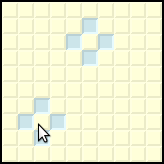
\includegraphics{img/Quinto-initialization}
  \caption{Quinto game at the beginning}
  \label{fig:quinto_beg}
\end{figure}

 \begin{figure}[ht]
  \centering
  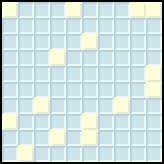
\includegraphics{img/Quinto-game}
  \caption{Quinto game execution}
  \label{fig:quinto_exec}
\end{figure}
 
  \end{description}
\end{enumerate}

\begin{thebibliography}{1}

\bibitem{krasner:bits_of_history}
Glenn Krasner; \textit{Smalltalk-80, Bits of History, Words of Advice}, 1982.

\bibitem{black:squeak_by_example}Andrew P. Black, Stéphane Ducasse,
Oscar Nierstrasz, Damien Pollet; \textit{Squeak by example}, 2009.

\bibitem{goldberg:blue_book}Adele Goldberg, David Robson; \textit{Blue Book},
1983.

\bibitem{gokel:comp_prog_using_gnu_smalltalk}Canol Gökel; \textit{Computer
Programming using GNU Smalltalk}, 2009.

\bibitem{web:squeak}Squeak website,
\verb|http://www.squeak.org|.

\bibitem{wiki:smalltalk}Wikipedia, The Free Encyclopedia,
\verb|http://en.wikipedia.org/wiki/Smalltalk|.

\bibitem{lp:insertion_sort}Literate
programs,
Insertion
sort;
\begin{verbatim}
http://en.literateprograms.org/
Insertion_sort_%28Smalltalk%29#chunk%20use:insertionSort.st
\end{verbatim}

\bibitem{ignalls:report}		
Dan Ingalls; \begin{verbatim}http://groups.google.com/
group/comp.lang.smalltalk/browse_thread/thread/
798b7a065f08bd7f/70e0d90098d816ef#70e0d90098d816ef
\end{verbatim}

\end{thebibliography}

\end{document}
